To determine if systematic uncertainties need to be accounted for in the \ZJETS and \ttbar normalization scale factors listed in Section~\ref{sec:BkgNorm}, each scale factor is studied, binned in \ST, \ptof{\PmuOne}, and \ptof{\jetOne}. The study was repeated for each year of data-taking, as shown in Figs.~\ref{figapp:sfstudy_2016}--\ref{figapp:sfstudy_2018}.

\begin{figure}[H]
    \centering
    {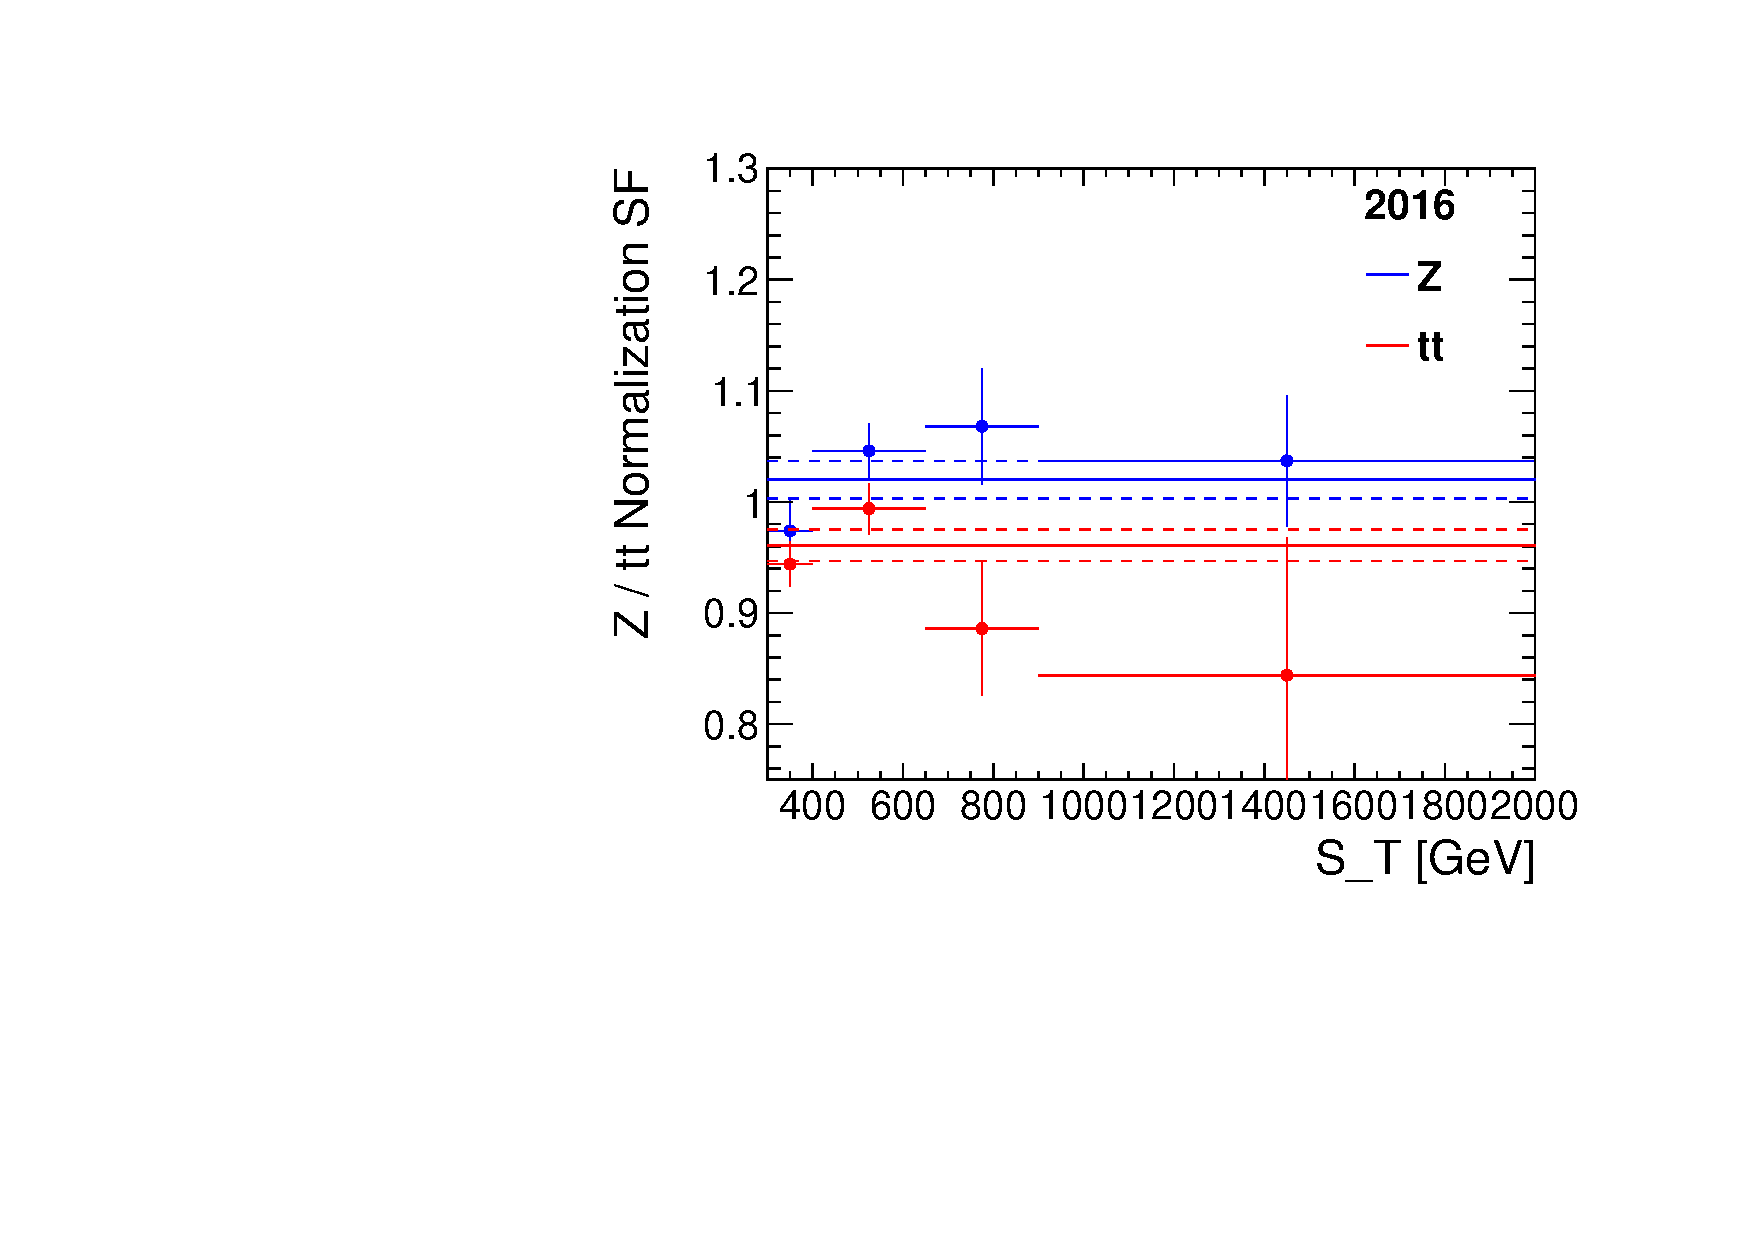
\includegraphics[width=.4\textwidth]{Images/Analysis/SFStudy/mumuScaleFactors_ST_2016.pdf}}
    {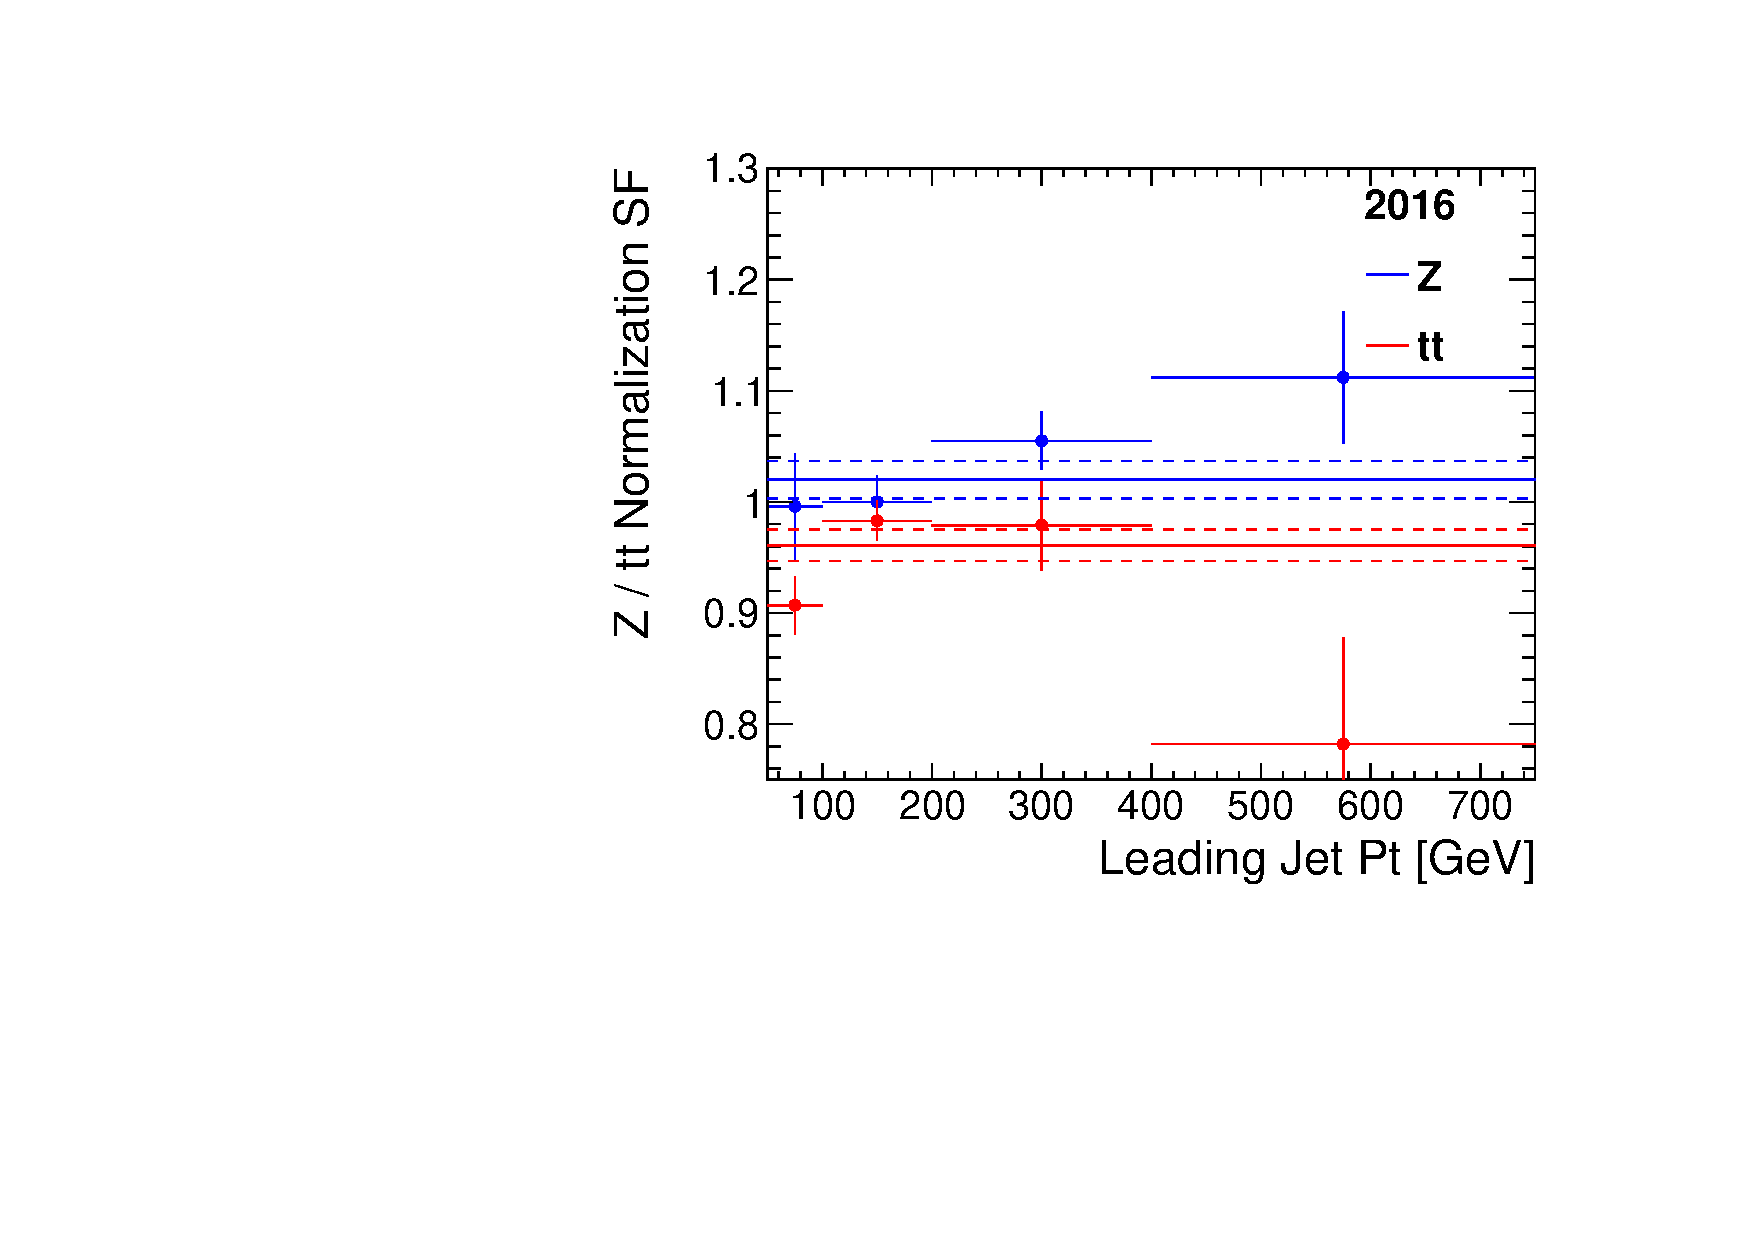
\includegraphics[width=.4\textwidth]{Images/Analysis/SFStudy/mumuScaleFactors_jetPt_2016.pdf}}
    {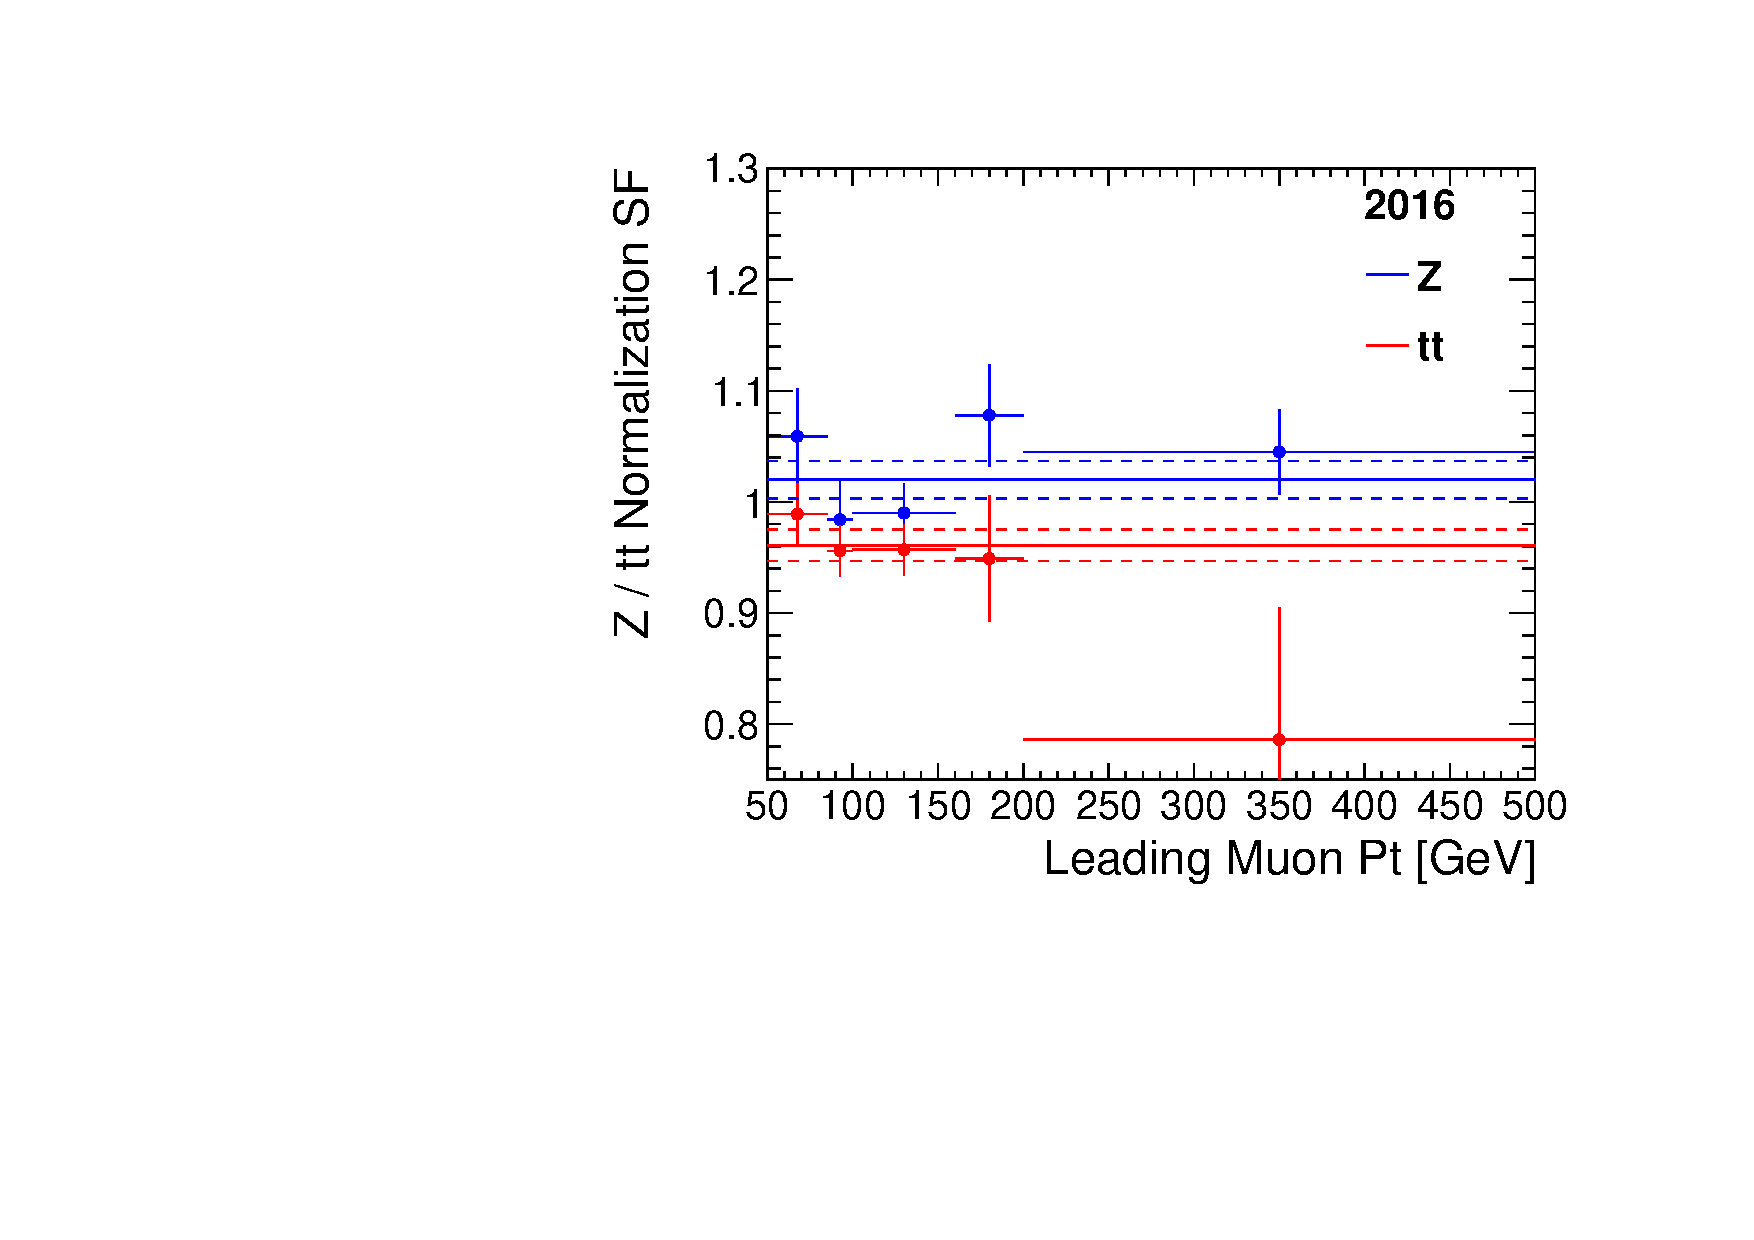
\includegraphics[width=.4\textwidth]{Images/Analysis/SFStudy/mumuScaleFactors_muPt_2016.pdf}}
    \caption{\ZJETS (red) and \ttbar (blue) normalization scale factors and their statistical uncertainties in bins of \ST (left), \ptof{\PmuOne} (center), and \ptof{\jetOne} (right) in the 2016 data-taking period. The inclusive scale factors are represented by a solid horizontal line, while statistical uncertainties on the inclusive scale factors are represented by dashed lines.}
    \label{figapp:sfstudy_2016}
\end{figure}

\begin{figure}[H]
    \centering
    {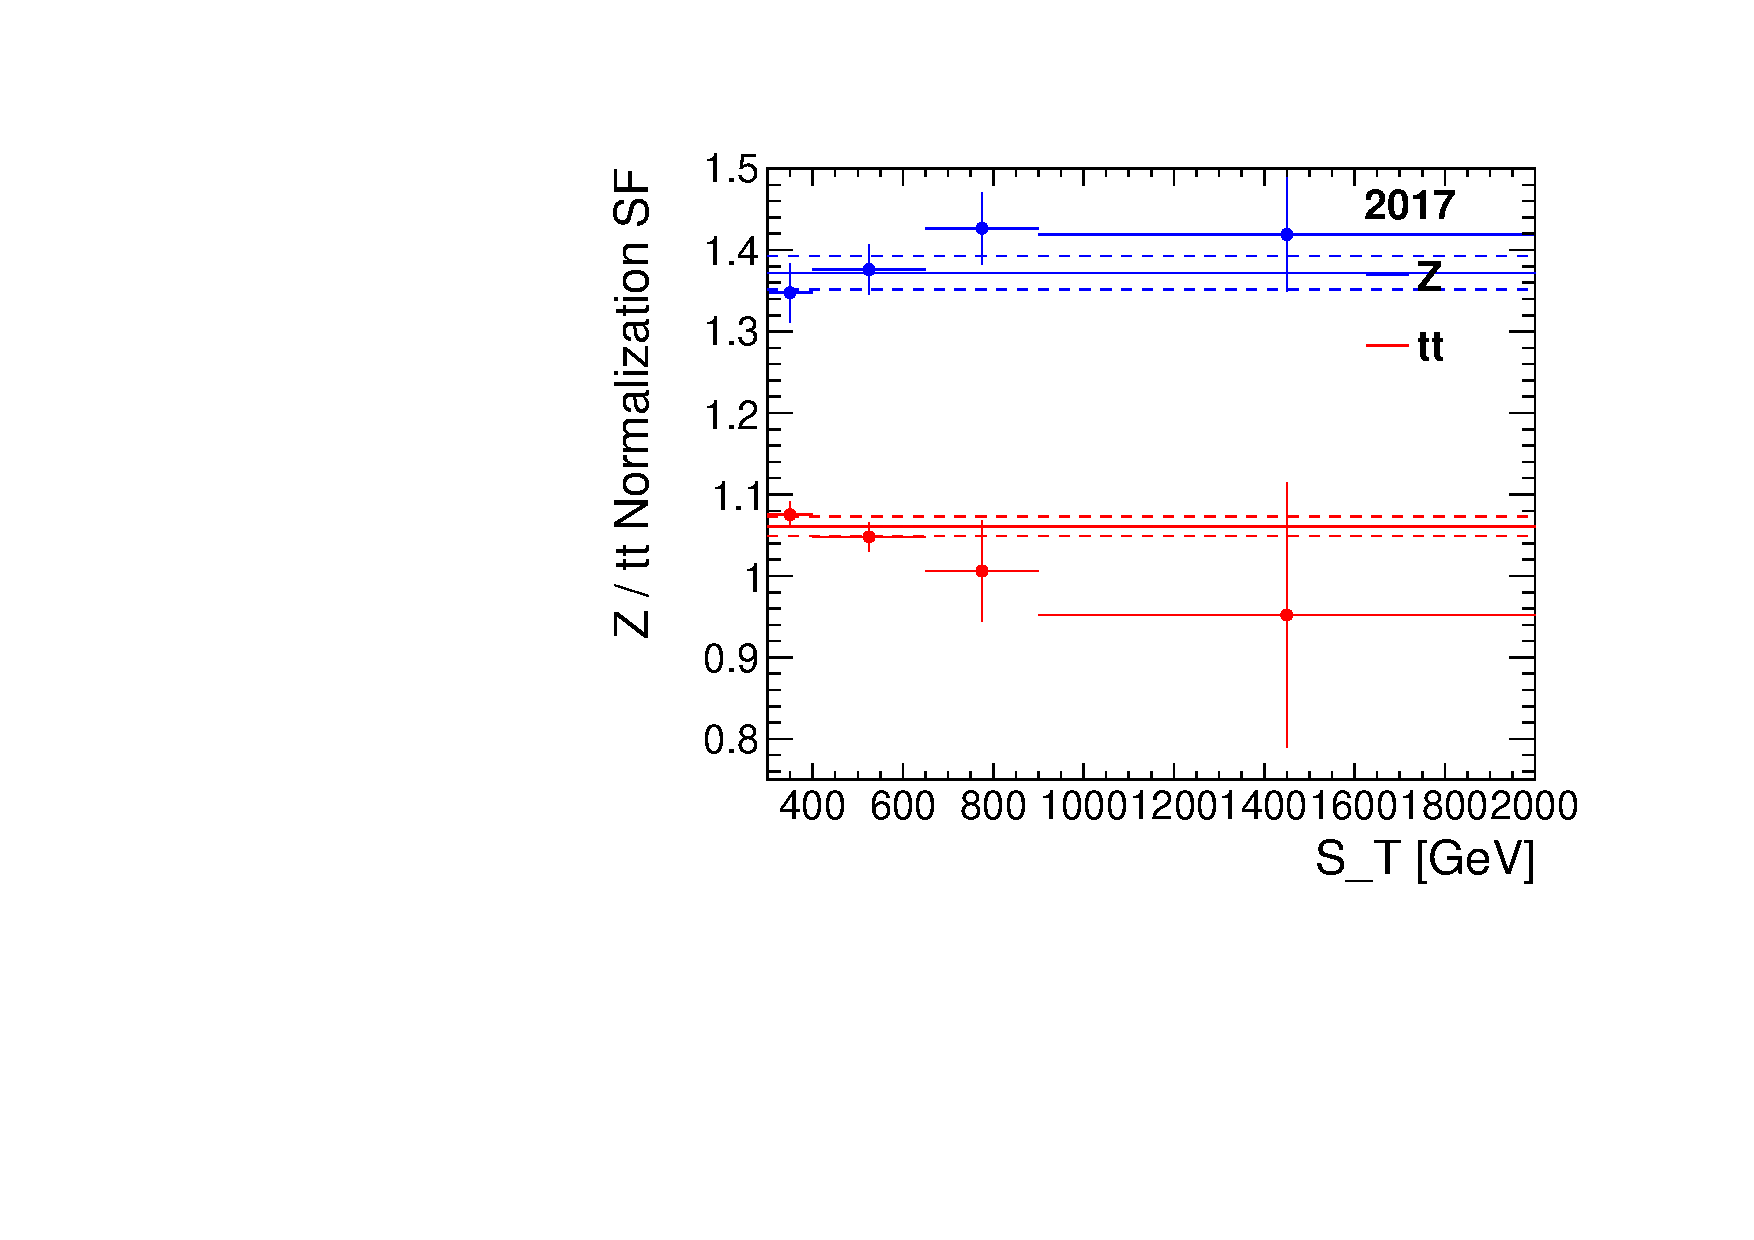
\includegraphics[width=.4\textwidth]{Images/Analysis/SFStudy/mumuScaleFactors_ST_2017.pdf}}
    {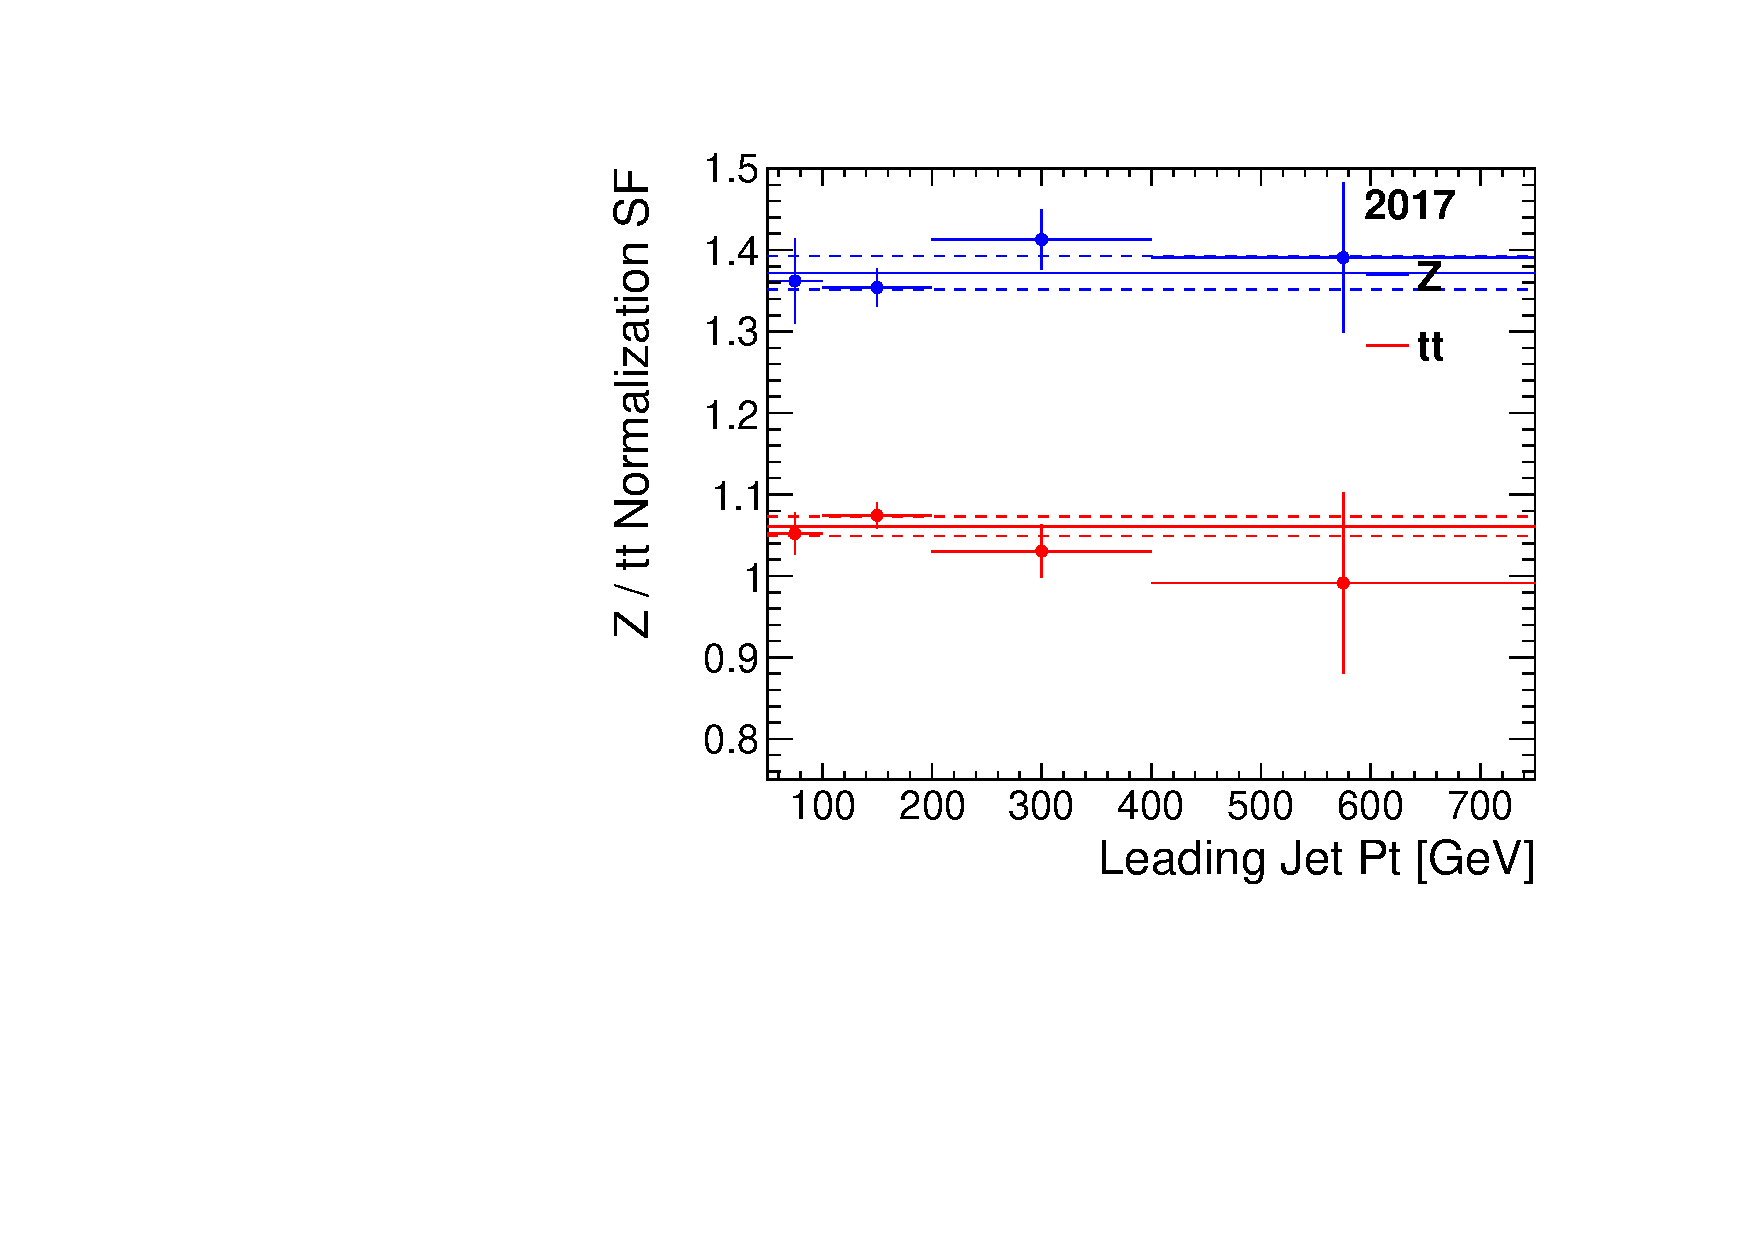
\includegraphics[width=.4\textwidth]{Images/Analysis/SFStudy/mumuScaleFactors_jetPt_2017.pdf}}
    {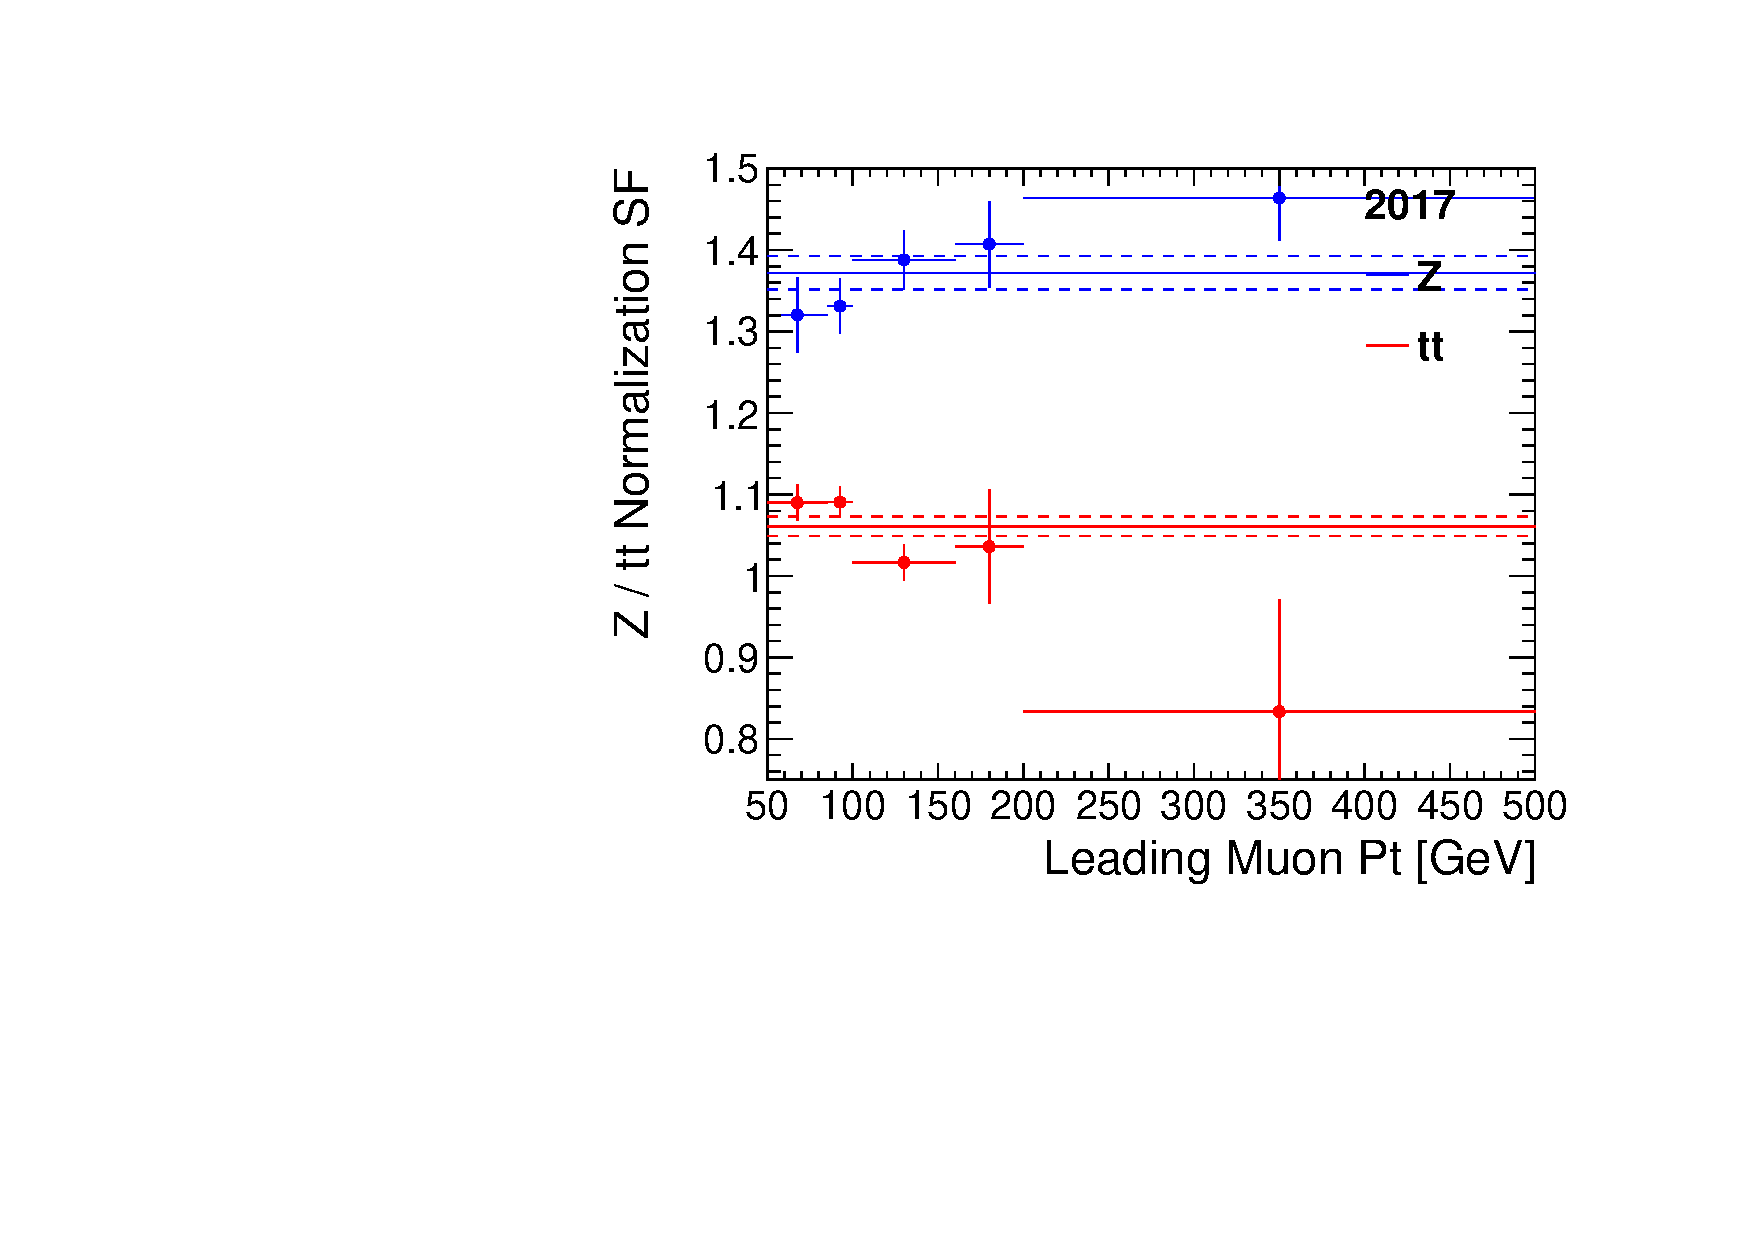
\includegraphics[width=.4\textwidth]{Images/Analysis/SFStudy/mumuScaleFactors_muPt_2017.pdf}}
    \caption{\ZJETS (red) and \ttbar (blue) normalization scale factors and their statistical uncertainties in bins of \ST (left), \ptof{\PmuOne} (center), and \ptof{\jetOne} (right) in the 2017 data-taking period. The inclusive scale factors are represented by a solid horizontal line, while statistical uncertainties on the inclusive scale factors are represented by dashed lines.}
    \label{figapp:sfstudy_2017}
\end{figure}

\begin{figure}[H]
    \centering
    {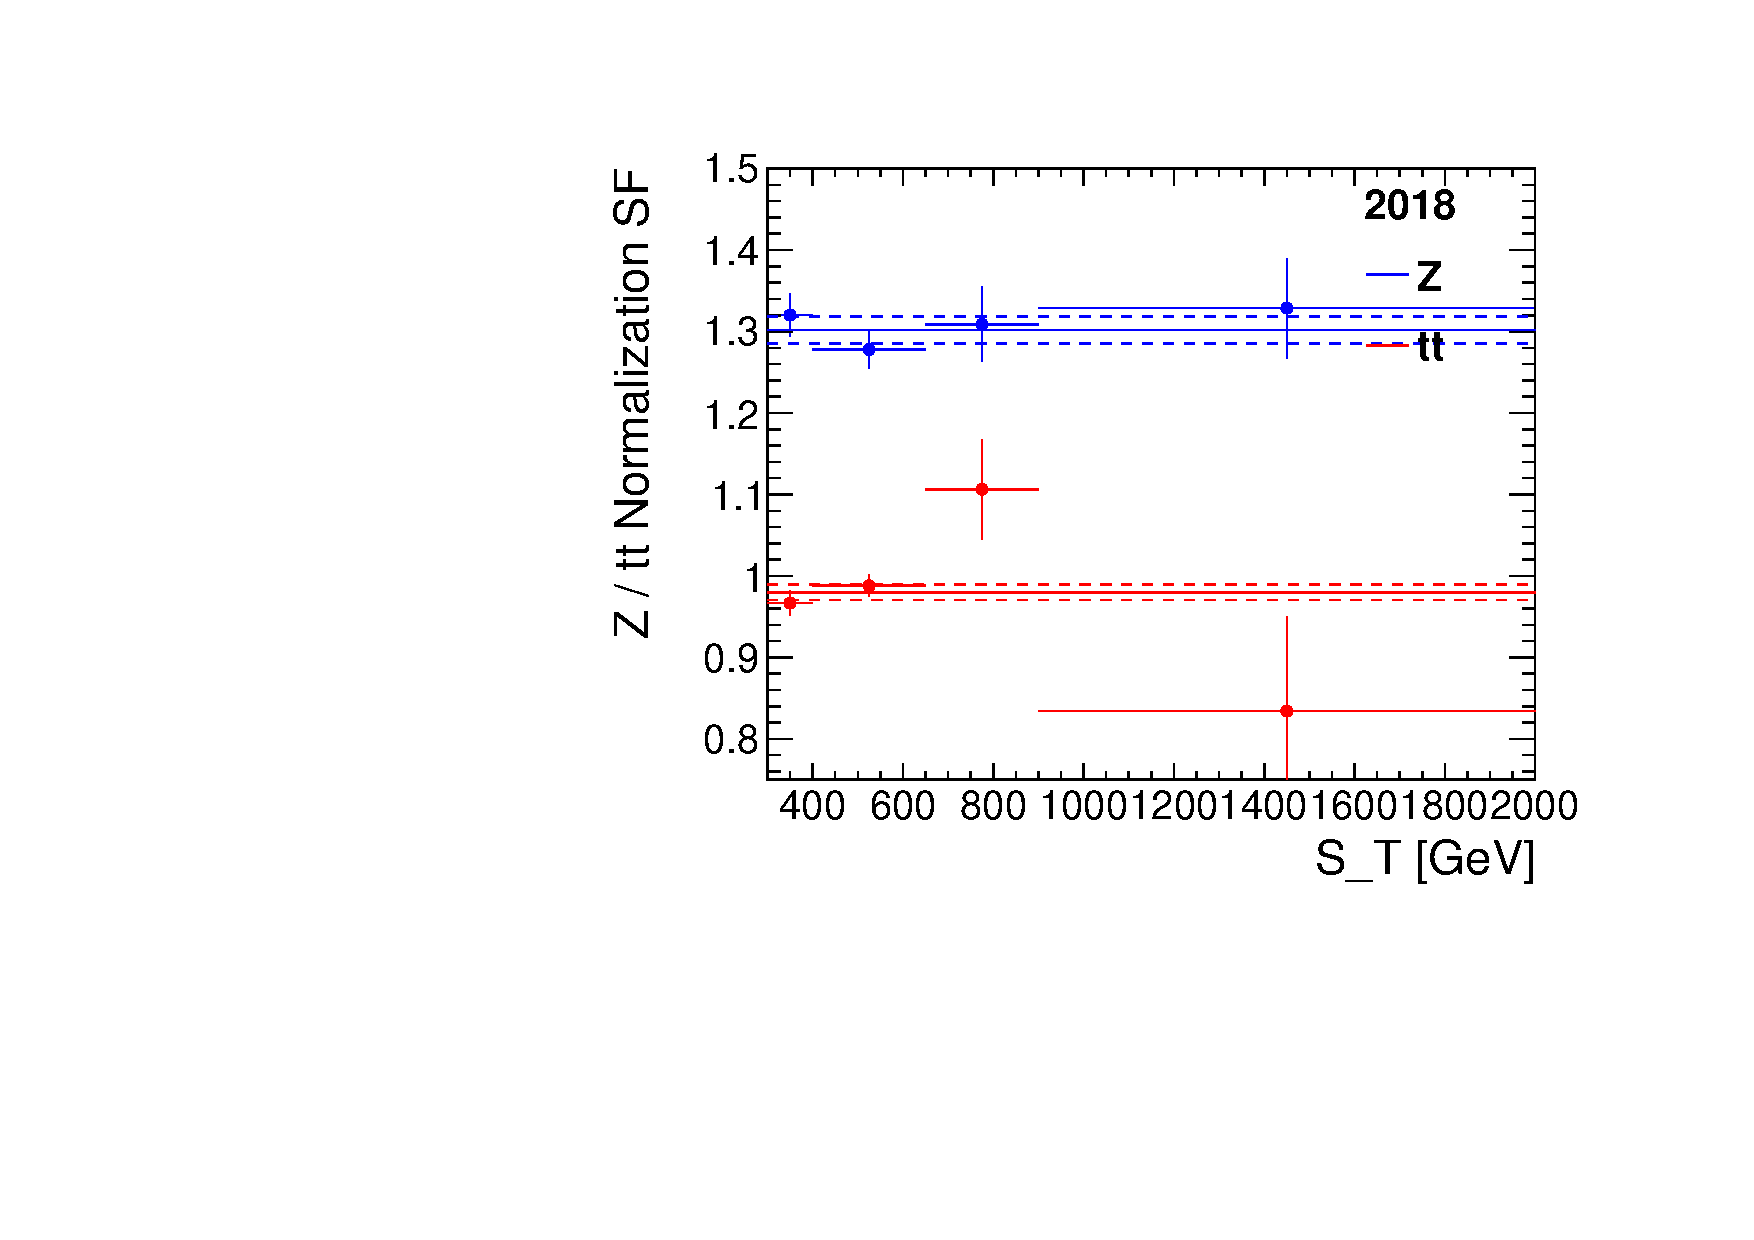
\includegraphics[width=.4\textwidth]{Images/Analysis/SFStudy/mumuScaleFactors_ST_2018.pdf}}
    {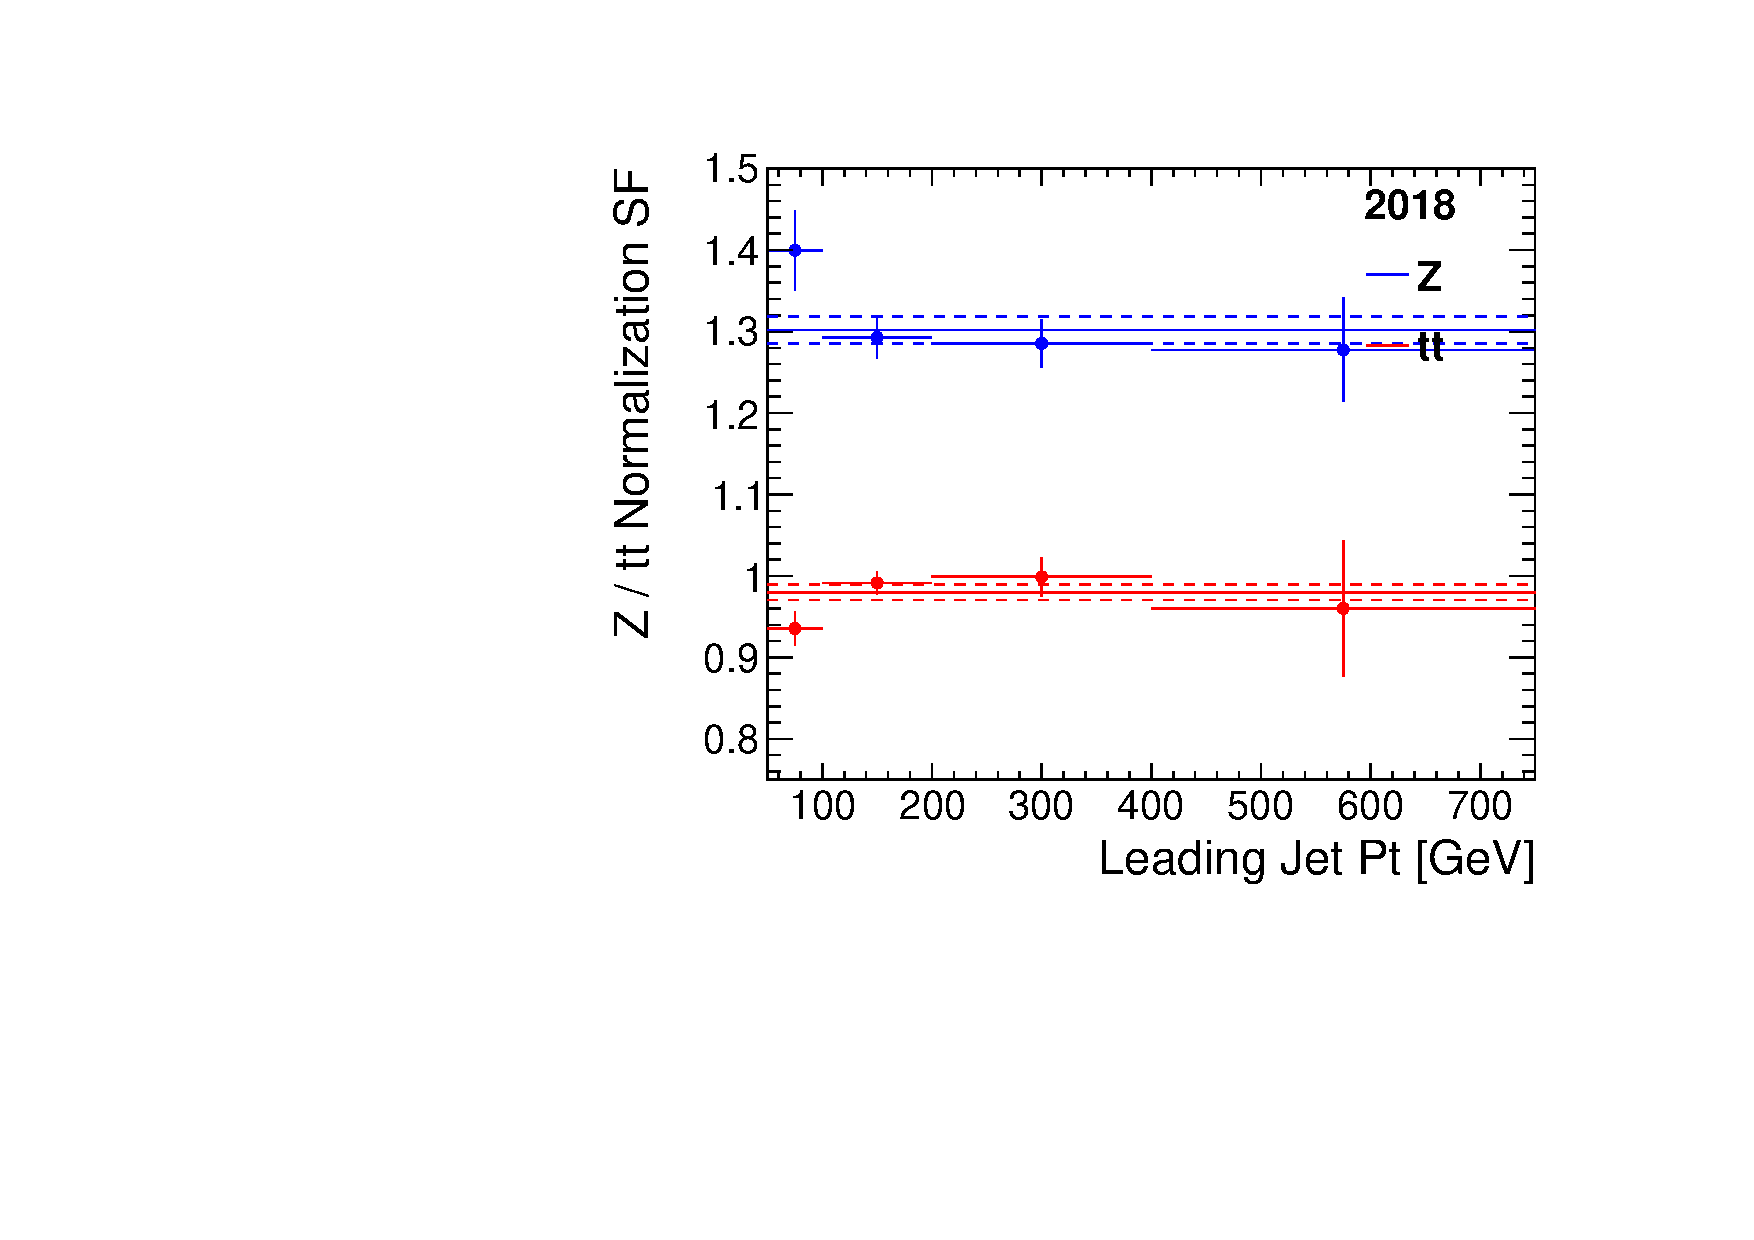
\includegraphics[width=.4\textwidth]{Images/Analysis/SFStudy/mumuScaleFactors_jetPt_2018.pdf}}
    {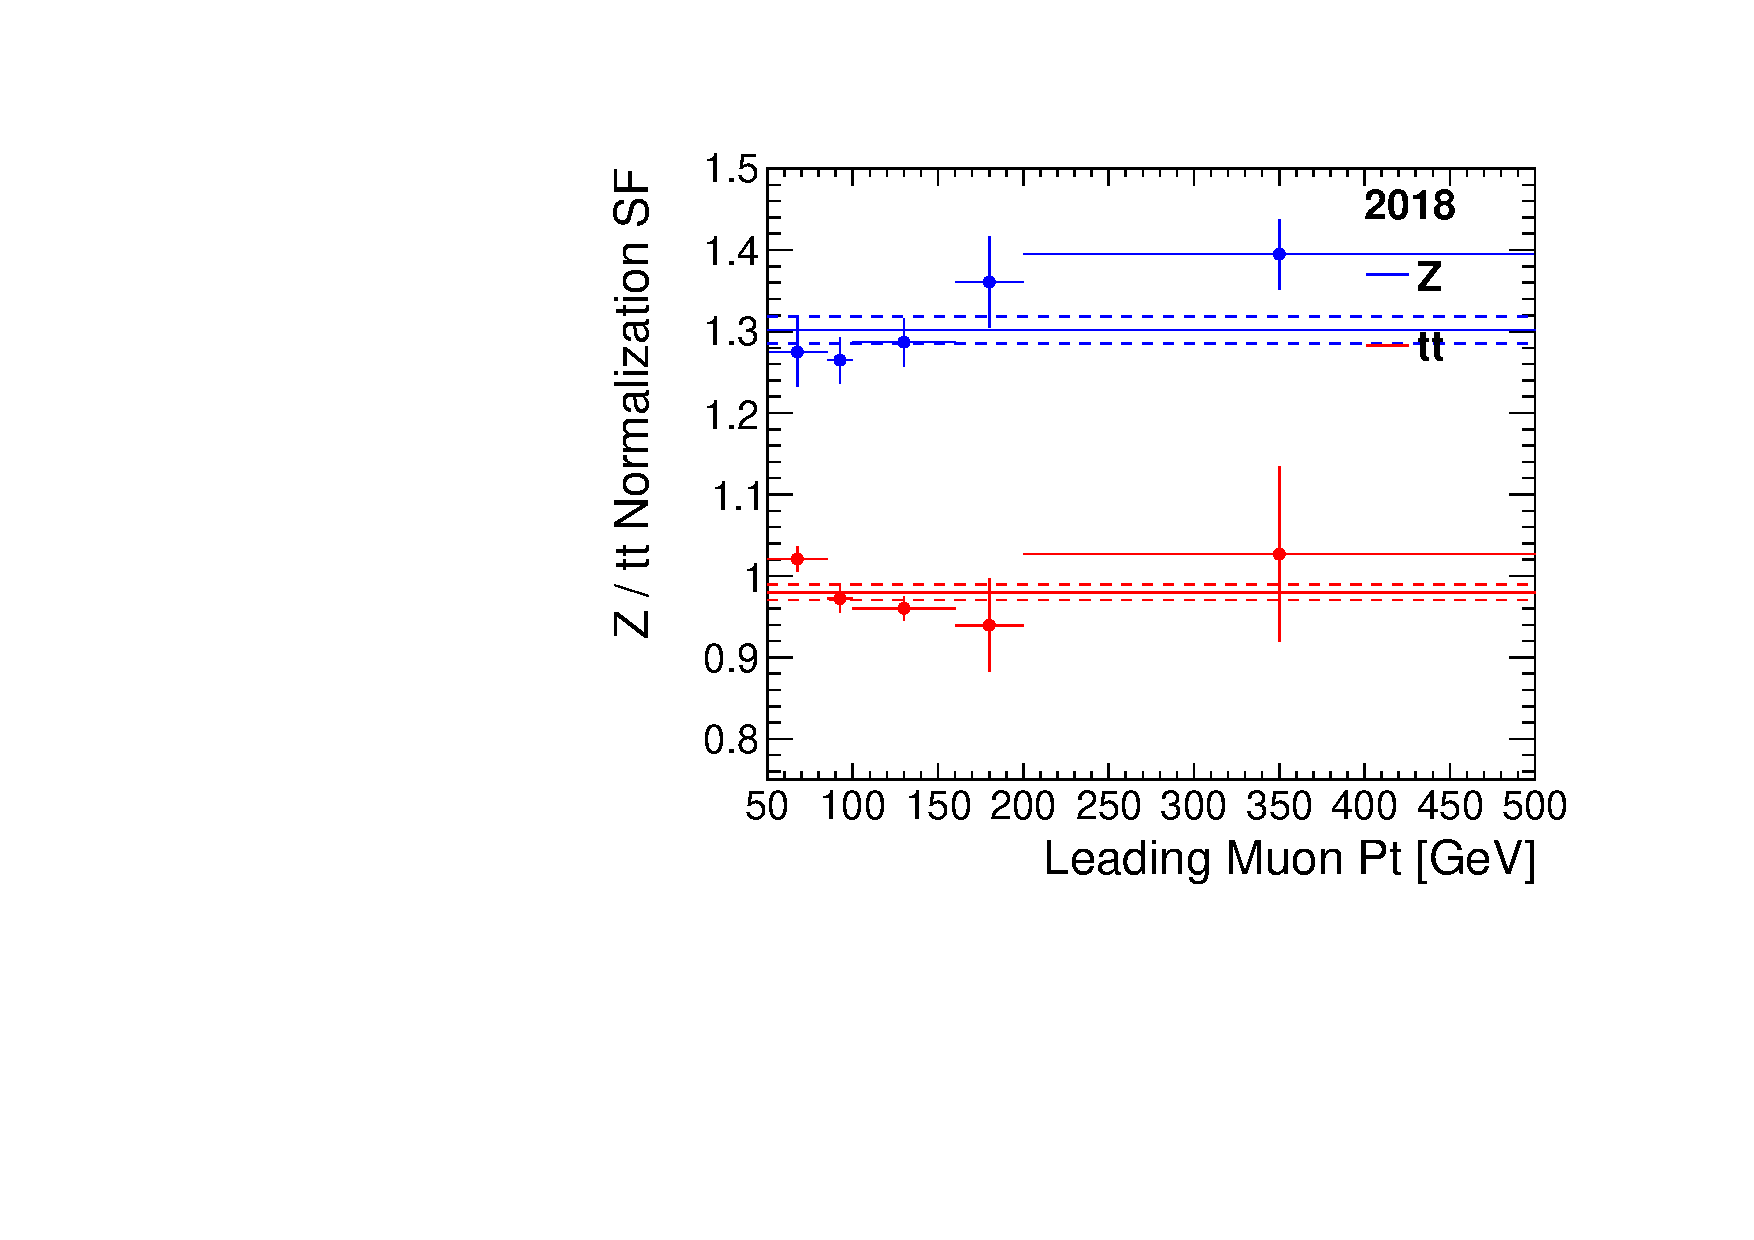
\includegraphics[width=.4\textwidth]{Images/Analysis/SFStudy/mumuScaleFactors_muPt_2018.pdf}}
    \caption{\ZJETS (red) and \ttbar (blue) normalization scale factors and their statistical uncertainties in bins of \ST (left), \ptof{\PmuOne} (center), and \ptof{\jetOne} (right) in the 2018 data-taking period. The inclusive scale factors are represented by a solid horizontal line, while statistical uncertainties on the inclusive scale factors are represented by dashed lines.}
    \label{figapp:sfstudy_2018}
\end{figure}

Also studied was the stability of the normalization scale factors with and without topPt reweighting. Shown in Figs.~\ref{figapp:sfstudy_st}--\ref{figapp:sfstudy_jetPt} are the comparisons without (left) and with (right) topPt reweighting. We in general see a better stability of the normalization scale factors after applying the topPt reweighting.

\begin{figure}[H]
    \centering
    {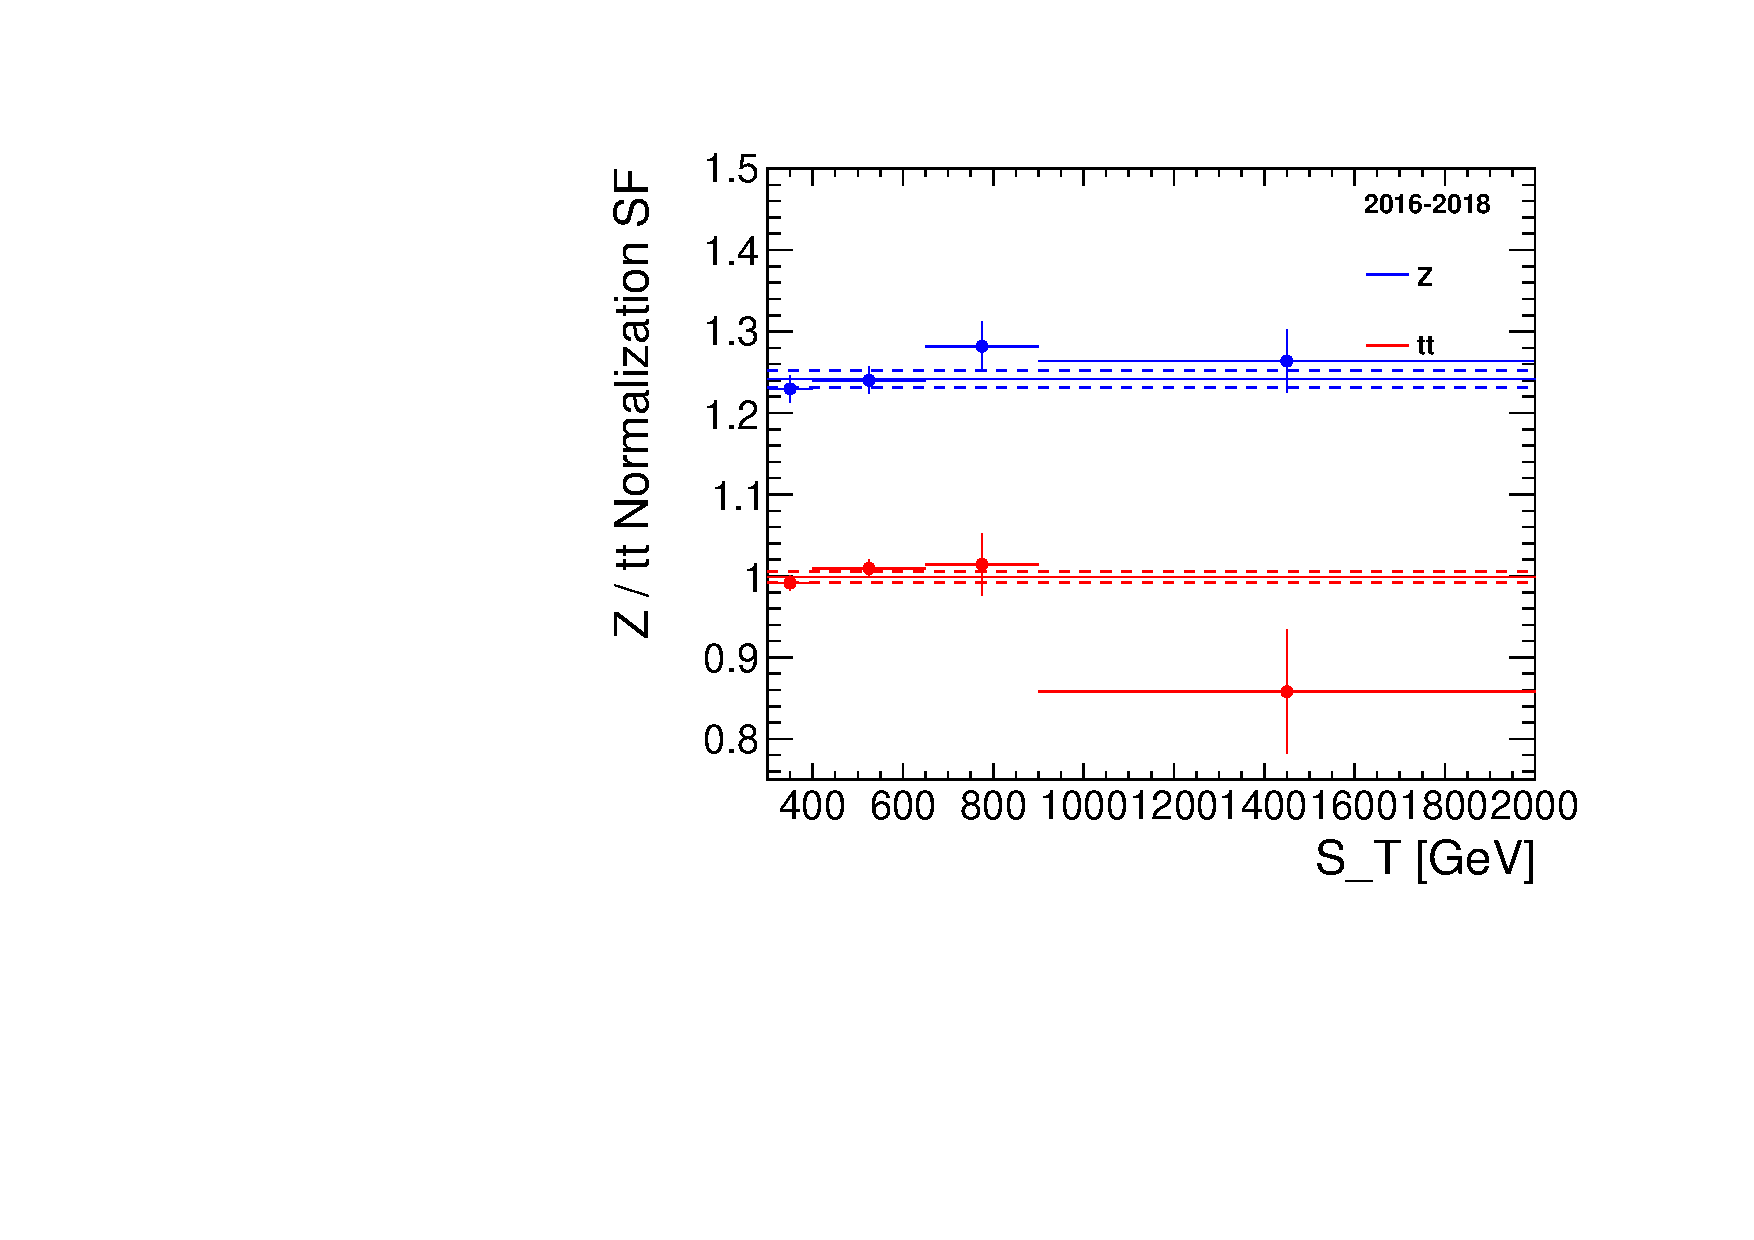
\includegraphics[width=.4\textwidth]{Images/Analysis/SFStudy/mumuScaleFactors_ST.pdf}}
    {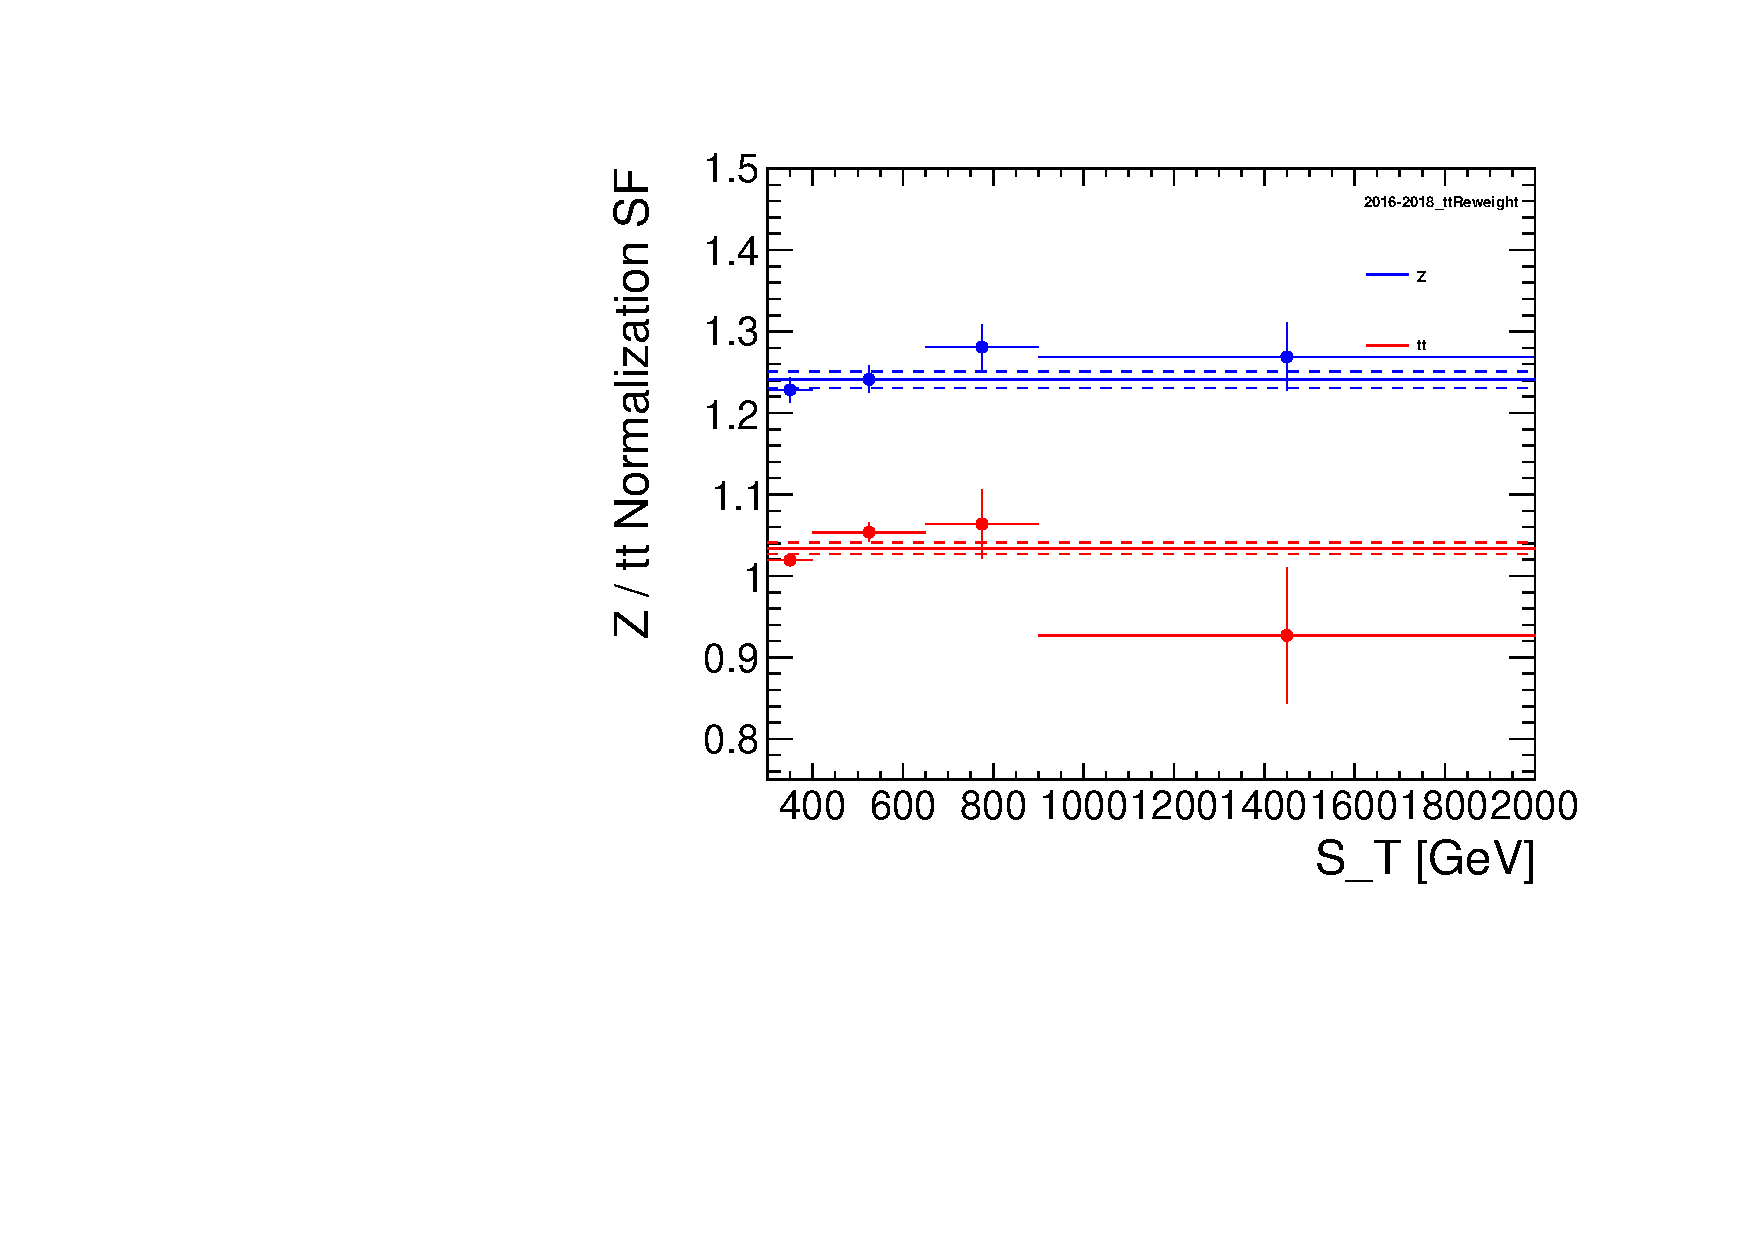
\includegraphics[width=.4\textwidth]{Images/Analysis/SFStudy/mumuScaleFactors_ST_topPt.pdf}}
    \caption{\ZJETS (red) and \ttbar (blue) normalization scale factors and their statistical uncertainties in bins of \ST without (left) and with (right) topPt reweighting in the 2016-2018 data-taking period. The inclusive scale factors are represented by a solid horizontal line, while statistical uncertainties on the inclusive scale factors are represented by dashed lines.}
    \label{figapp:sfstudy_st}
\end{figure}

\begin{figure}[H]
    \centering
    {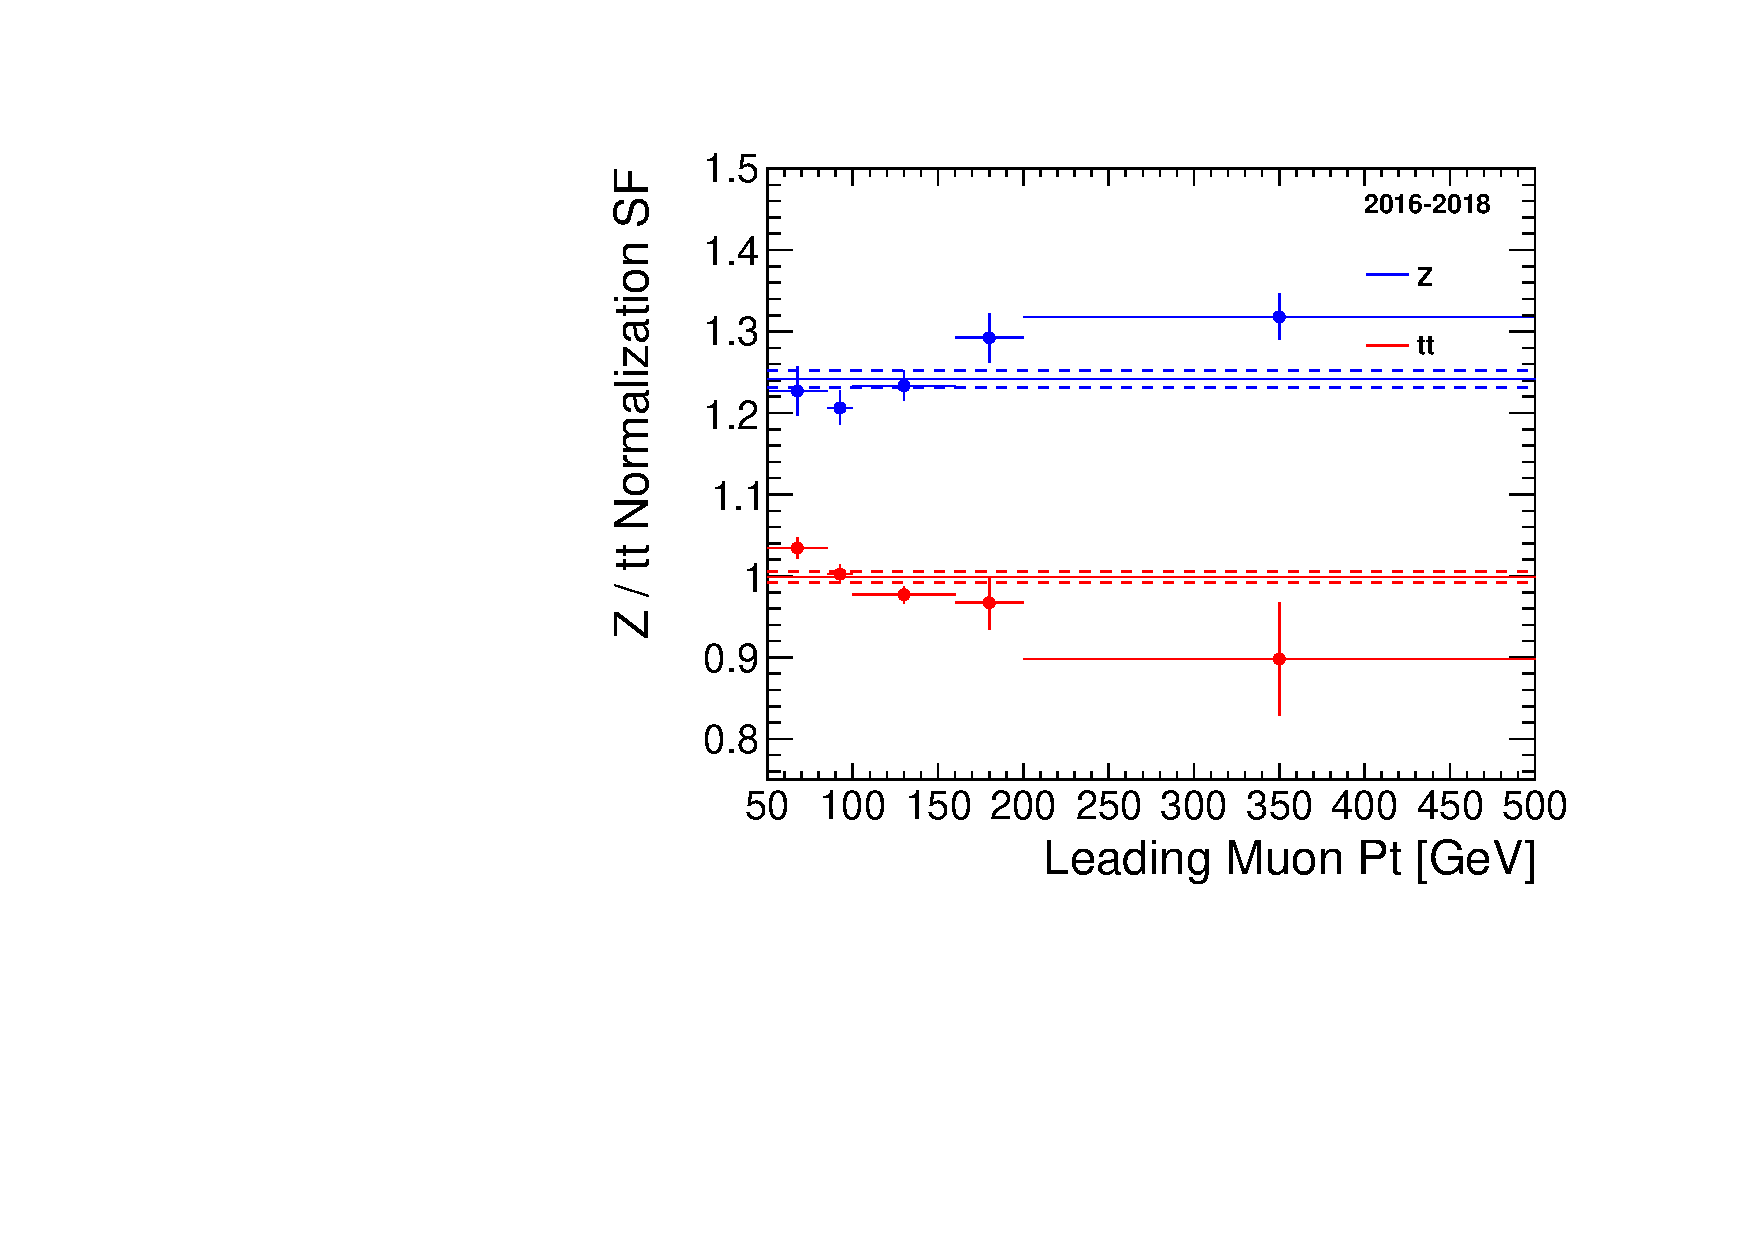
\includegraphics[width=.4\textwidth]{Images/Analysis/SFStudy/mumuScaleFactors_muPt.pdf}}
    {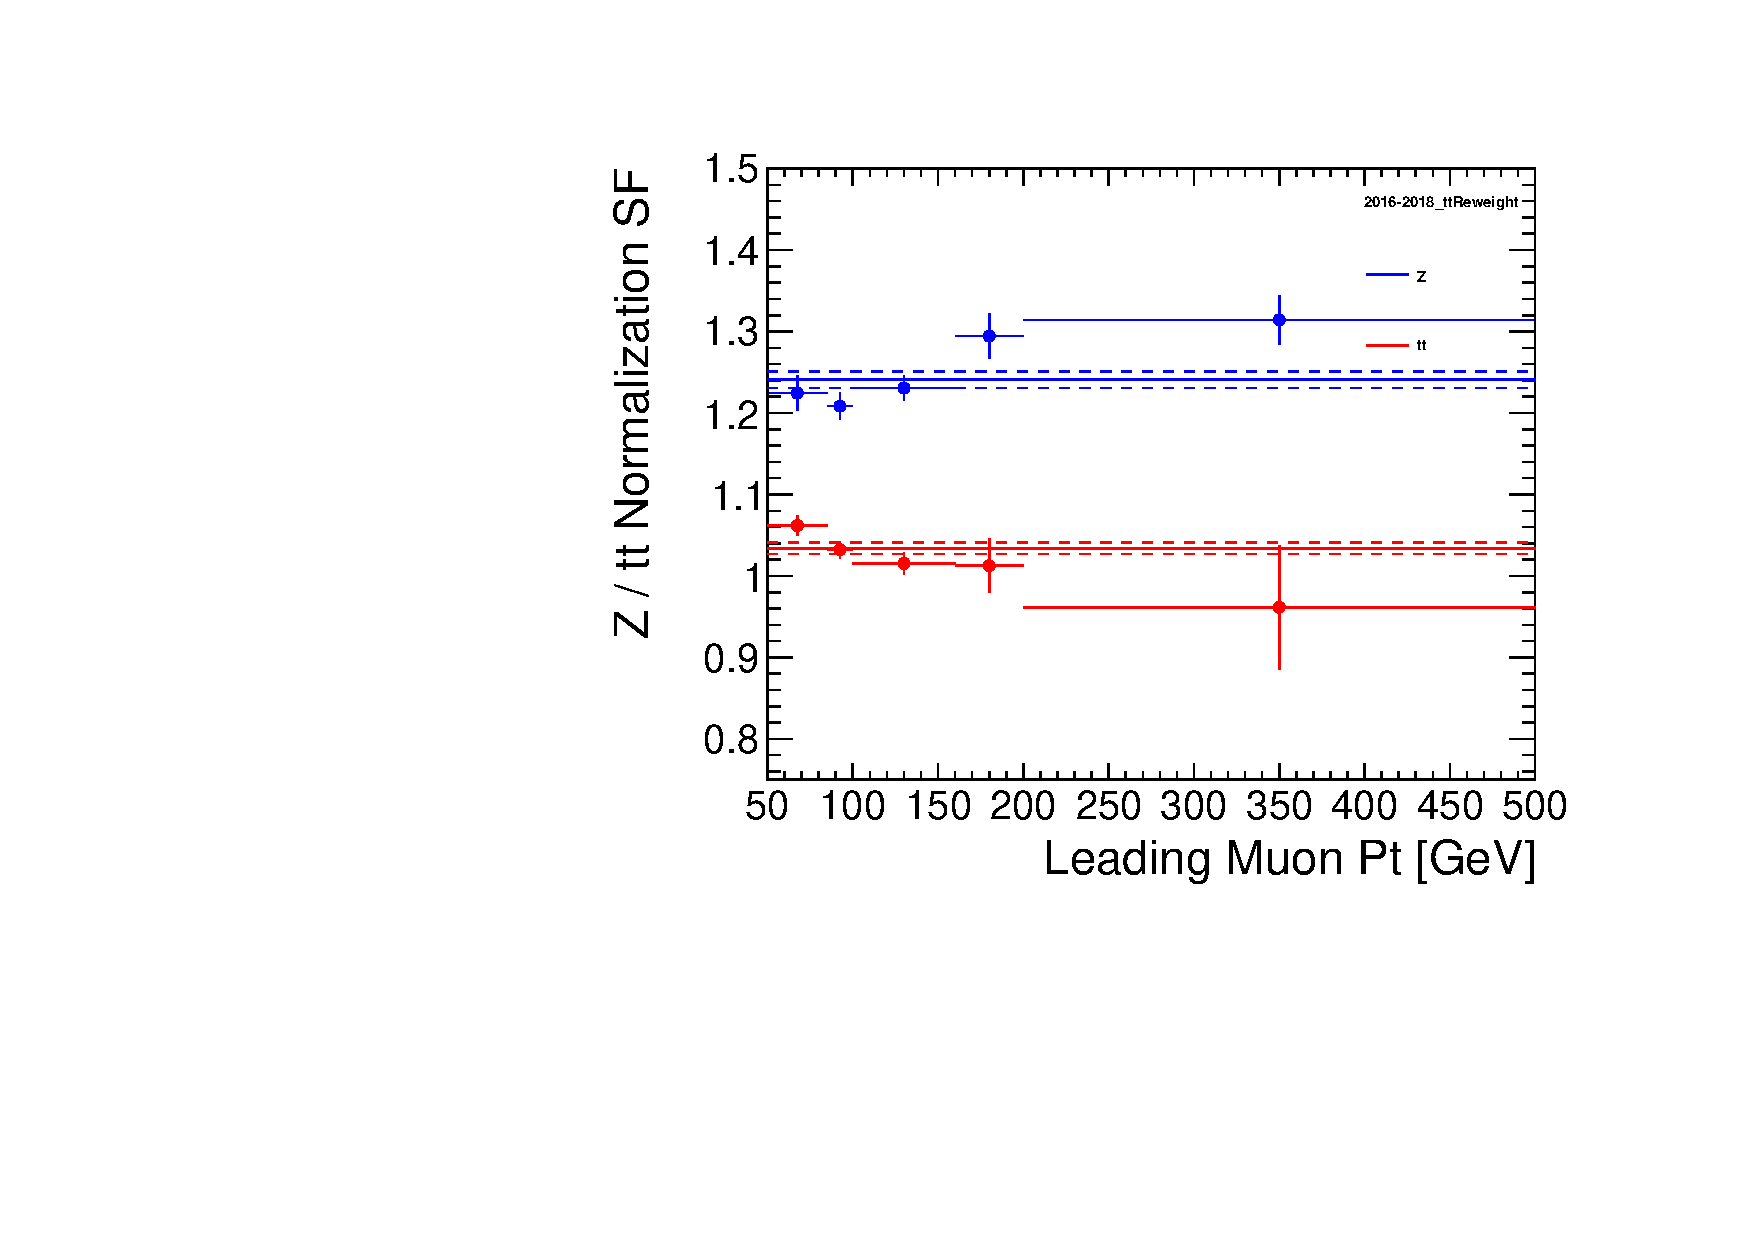
\includegraphics[width=.4\textwidth]{Images/Analysis/SFStudy/mumuScaleFactors_muPt_topPt.pdf}}
    \caption{\ZJETS (red) and \ttbar (blue) normalization scale factors and their statistical uncertainties in bins of \ptof{\PmuOne} without (left) and with (right) topPt reweighting in the 2016-2018 data-taking period. The inclusive scale factors are represented by a solid horizontal line, while statistical uncertainties on the inclusive scale factors are represented by dashed lines.}
    \label{figapp:sfstudy_muPt}
\end{figure}

\begin{figure}[H]
    \centering
    {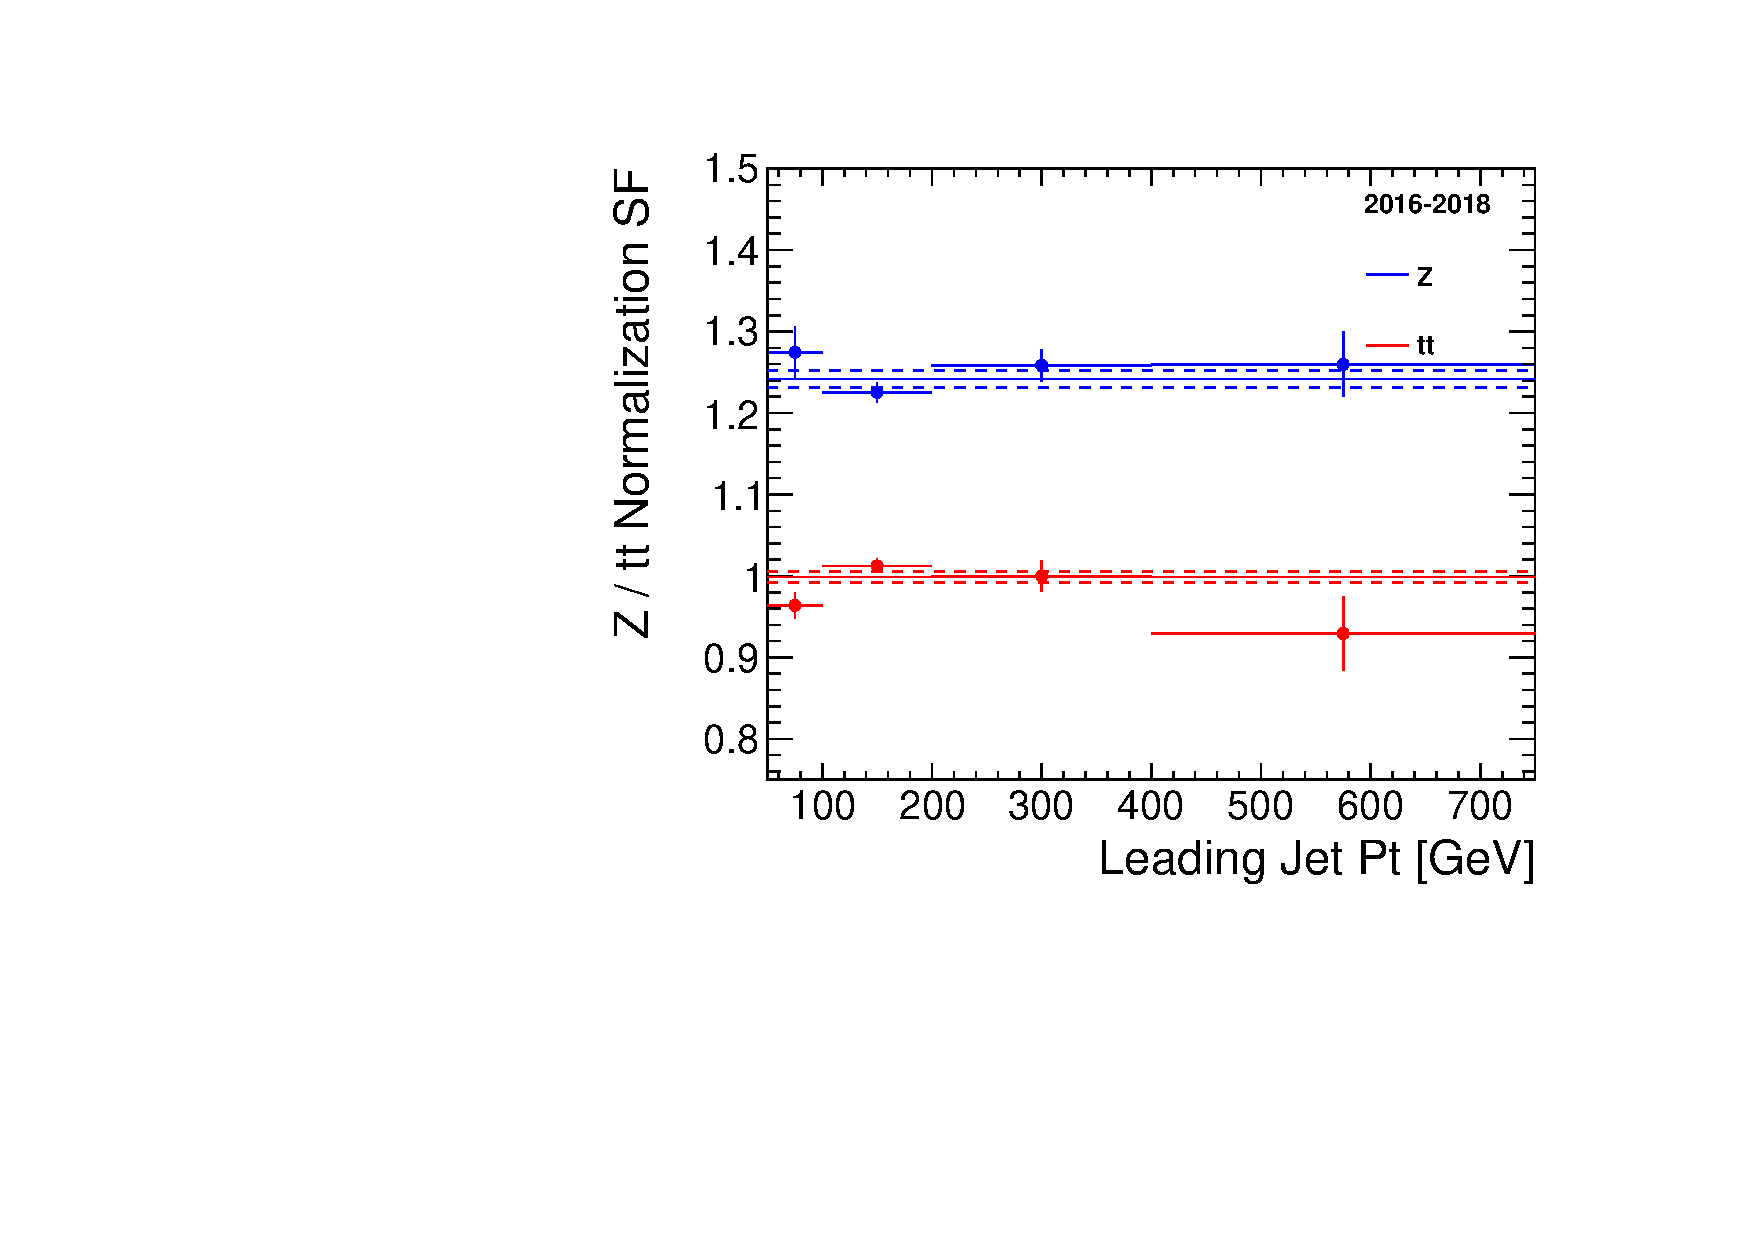
\includegraphics[width=.4\textwidth]{Images/Analysis/SFStudy/mumuScaleFactors_jetPt.pdf}}
    {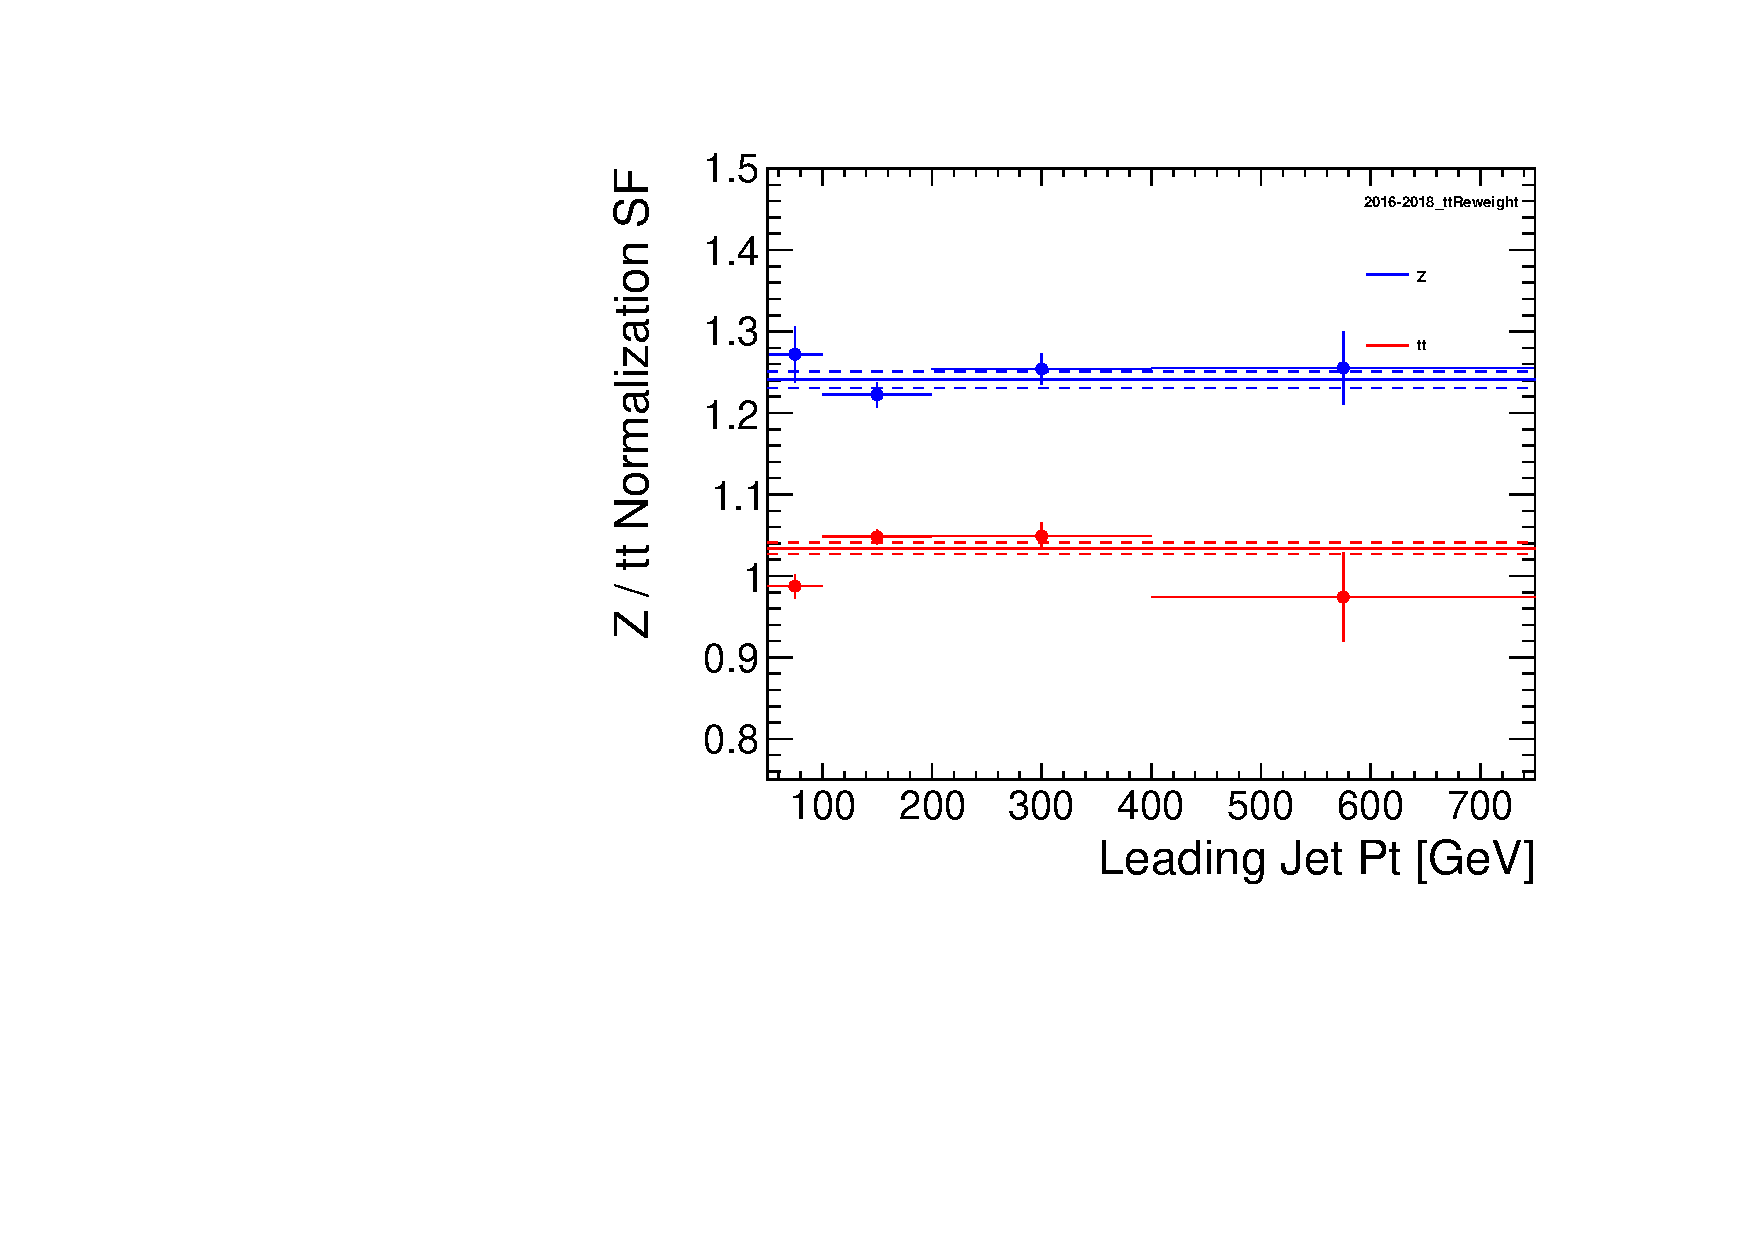
\includegraphics[width=.4\textwidth]{Images/Analysis/SFStudy/mumuScaleFactors_jetPt_topPt.pdf}}
    \caption{\ZJETS (red) and \ttbar (blue) normalization scale factors and their statistical uncertainties in bins of \ptof{\jetOne} without (left) and with (right) topPt reweighting in the 2016-2018 data-taking period. The inclusive scale factors are represented by a solid horizontal line, while statistical uncertainties on the inclusive scale factors are represented by dashed lines.}
    \label{figapp:sfstudy_jetPt}
\end{figure}

To ensure that systematic uncertainties originating from single top, W+Jets, \TTV, and diboson MC do not translate to the Z+Jets and \ttbar normalization scale factors, the ``other'' background simulations were varied $\SI{\pm20}{\%}$. Even with these variations, the background normalization scale factors agree within their errors. Table~\ref{tab:sfvariations} lists the background scale factors given each variation of the ``other'' backgrounds.

\begin{table}[htb]
    \caption{Background normalization scale factors for each variation in ``other'' backgrounds.}
    \begin{center}
           %\scriptsize
           \begin{tabular}{cccccc}\hline\hline
                \multicolumn{3}{c}{\RZ}                                         &	\multicolumn{3}{c}{\RTT} \\\hline
                variation 	                &   scale factor    &   error \stat &   variation	                &   scale factor    &   error \stat \\ \hline
                Nominal	                    &   1.017	        &   0.017	    &   Nominal	                    &   1.003	        &   0.014 \\
                $\text{Other}+\SI{10}{\%}$  &   1.012	        &   0.017	    &   $\text{Other}+\SI{10}{\%}$	&   1.002	        &   0.014 \\
                $\text{Other}-\SI{10}{\%}$  &   1.022	        &   0.017	    &   $\text{Other}-\SI{10}{\%}$	&   1.004	        &   0.014 \\
                $\text{Other}+\SI{20}{\%}$  &   1.006	        &   0.017	    &   $\text{Other}+\SI{20}{\%}$	&   1.001	        &   0.014 \\
                $\text{Other}-\SI{20}{\%}$  &   1.027           &   0.017       &   $\text{Other}-\SI{20}{\%}$  &   1.005           &   0.014 \\ \hline \hline
            \end{tabular}
            \label{tab:sfvariations}
     \end{center}
 \end{table}
